\documentclass[twoside]{article}

\usepackage{aistats2021}
\usepackage{graphicx}
% If your paper is accepted, change the options for the package
% aistats2021 as follows:
%
%\usepackage[accepted]{aistats2021}
%
% This option will print headings for the title of your paper and
% headings for the authors names, plus a copyright note at the end of
% the first column of the first page.

% If you set papersize explicitly, activate the following three lines:
%\special{papersize = 8.5in, 11in}
%\setlength{\pdfpageheight}{11in}
%\setlength{\pdfpagewidth}{8.5in}

% If you use natbib package, activate the following three lines:
%\usepackage[round]{natbib}
%\renewcommand{\bibname}{References}
%\renewcommand{\bibsection}{\subsubsection*{\bibname}}

% If you use BibTeX in apalike style, activate the following line:
%\bibliographystyle{apalike}

\begin{document}

% If your paper is accepted and the title of your paper is very long,
% the style will print as headings an error message. Use the following
% command to supply a shorter title of your paper so that it can be
% used as headings.
%
%\runningtitle{I use this title instead because the last one was very long}

% If your paper is accepted and the number of authors is large, the
% style will print as headings an error message. Use the following
% command to supply a shorter version of the authors names so that
% they can be used as headings (for example, use only the surnames)
%
%\runningauthor{Surname 1, Surname 2, Surname 3, ...., Surname n}

\twocolumn[

\aistatstitle{Instructions for Paper Submissions to AISTATS 2021}

\aistatsauthor{ Author 1 \And Author 2 \And  Author 3 }

\aistatsaddress{ Institution 1 \And  Institution 2 \And Institution 3 } ]

\begin{abstract}
  The Abstract paragraph should be indented 0.25 inch (1.5 picas) on
  both left and right-hand margins. Use 10~point type, with a vertical
  spacing of 11~points. The \textbf{Abstract} heading must be centered,
  bold, and in point size 12. Two line spaces precede the
  Abstract. The Abstract must be limited to one paragraph.
\end{abstract}

\section{GENERAL FORMATTING INSTRUCTIONS}

The camera-ready versions of the accepted papers are 8 pages,
plus any additional pages needed for references.

Papers are in 2 columns with the overall line width of 6.75~inches (41~picas).
Each column is 3.25~inches wide (19.5~picas).  The space
between the columns is .25~inches wide (1.5~picas).  The left margin is 0.88~inches (5.28~picas).
Use 10~point type with a vertical spacing of
11~points. Please use US Letter size paper instead of A4.

Paper title is 16~point, caps/lc, bold, centered between 2~horizontal rules.
Top rule is 4~points thick and bottom rule is 1~point thick.
Allow 1/4~inch space above and below title to rules.

Author descriptions are center-justified, initial caps.  The lead
author is to be listed first (left-most), and the Co-authors are set
to follow.  If up to three authors, use a single row of author
descriptions, each one center-justified, and all set side by side;
with more authors or unusually long names or institutions, use more
rows.

Use one-half line space between paragraphs, with no indent.

\section{FIRST LEVEL HEADINGS}

First level headings are all caps, flush left, bold, and in point size
12. Use one line space before the first level heading and one-half line space
after the first level heading.

\subsection{Second Level Heading}

Second level headings are initial caps, flush left, bold, and in point
size 10. Use one line space before the second level heading and one-half line
space after the second level heading.

\subsubsection{Third Level Heading}

Third level headings are flush left, initial caps, bold, and in point
size 10. Use one line space before the third level heading and one-half line
space after the third level heading.

\paragraph{Fourth Level Heading}

Fourth level headings must be flush left, initial caps, bold, and
Roman type.  Use one line space before the fourth level heading, and
place the section text immediately after the heading with no line
break, but an 11 point horizontal space.

%%%
\subsection{Citations, Figure, References}


\subsubsection{Citations in Text}

Citations within the text should include the author's last name and
year, e.g., (Cheesman, 1985). 
%Apart from including the author's last name and year, citations can follow any style, as long as the style is consistent throughout the paper.  
Be sure that the sentence reads
correctly if the citation is deleted: e.g., instead of ``As described
by (Cheesman, 1985), we first frobulate the widgets,'' write ``As
described by Cheesman (1985), we first frobulate the widgets.''


The references listed at the end of the paper can follow any style as long as it is used consistently.

%Be sure to avoid
%accidentally disclosing author identities through citations.

\subsubsection{Footnotes}

Indicate footnotes with a number\footnote{Sample of the first
  footnote.} in the text. Use 8 point type for footnotes. Place the
footnotes at the bottom of the column in which their markers appear,
continuing to the next column if required. Precede the footnote
section of a column with a 0.5 point horizontal rule 1~inch (6~picas)
long.\footnote{Sample of the second footnote.}

\subsubsection{Figures}

All artwork must be centered, neat, clean, and legible.  All lines
should be very dark for purposes of reproduction, and art work should
not be hand-drawn.  Figures may appear at the top of a column, at the
top of a page spanning multiple columns, inline within a column, or
with text wrapped around them, but the figure number and caption
always appear immediately below the figure.  Leave 2 line spaces
between the figure and the caption. The figure caption is initial caps
and each figure should be numbered consecutively.

Make sure that the figure caption does not get separated from the
figure. Leave extra white space at the bottom of the page rather than
splitting the figure and figure caption.


\begin{figure}[thb]
	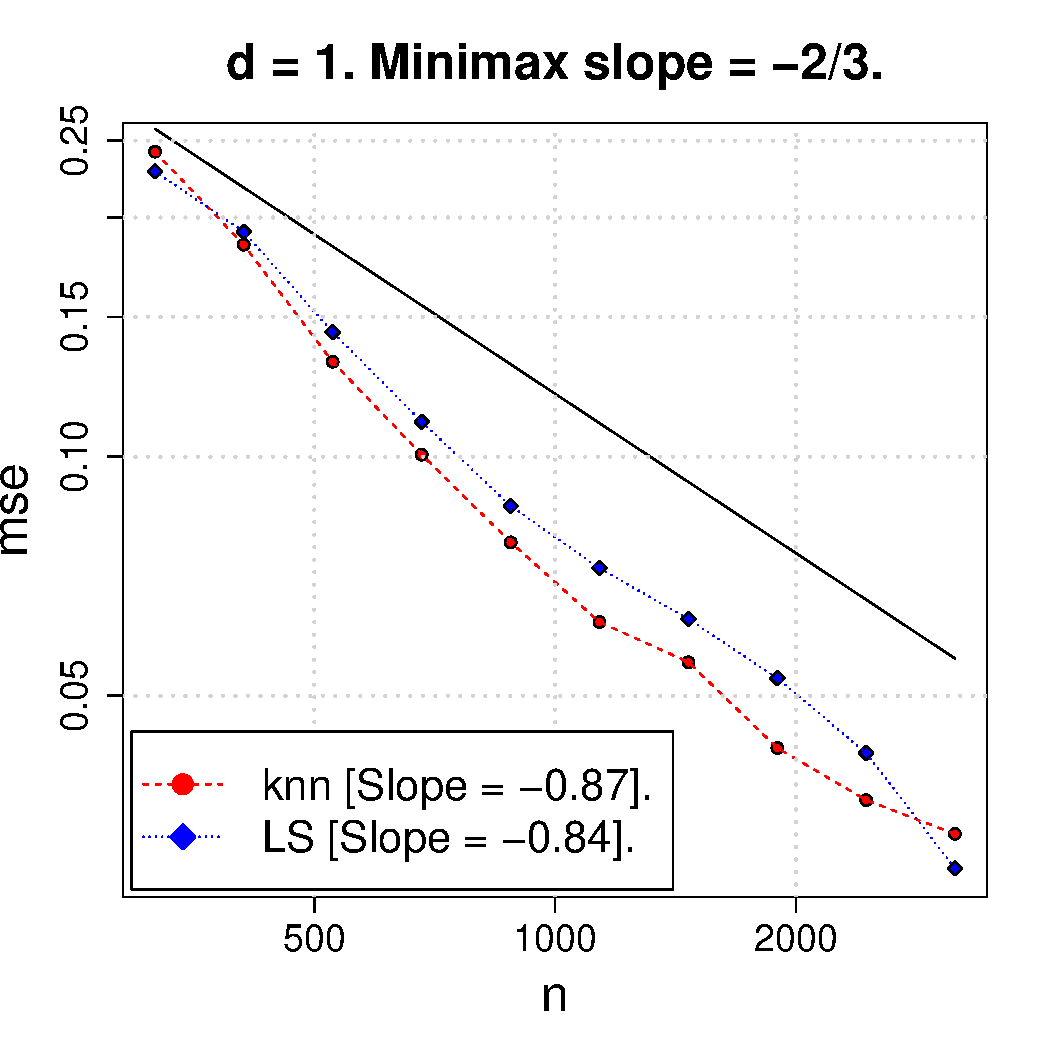
\includegraphics[width=.23\textwidth]{figures/mse_by_sample_size_1d.pdf}
	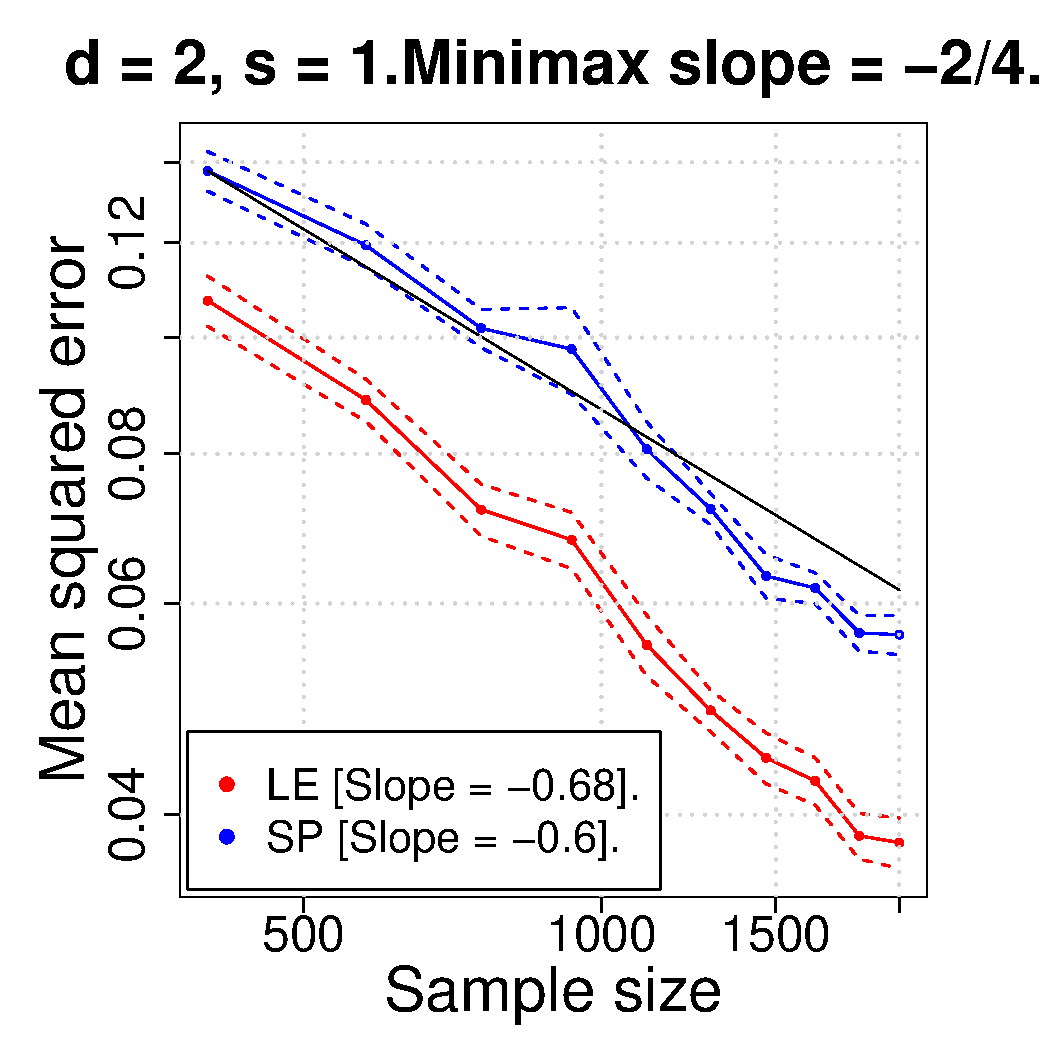
\includegraphics[width=.23\textwidth]{figures/mse_by_sample_size_2d.pdf}
	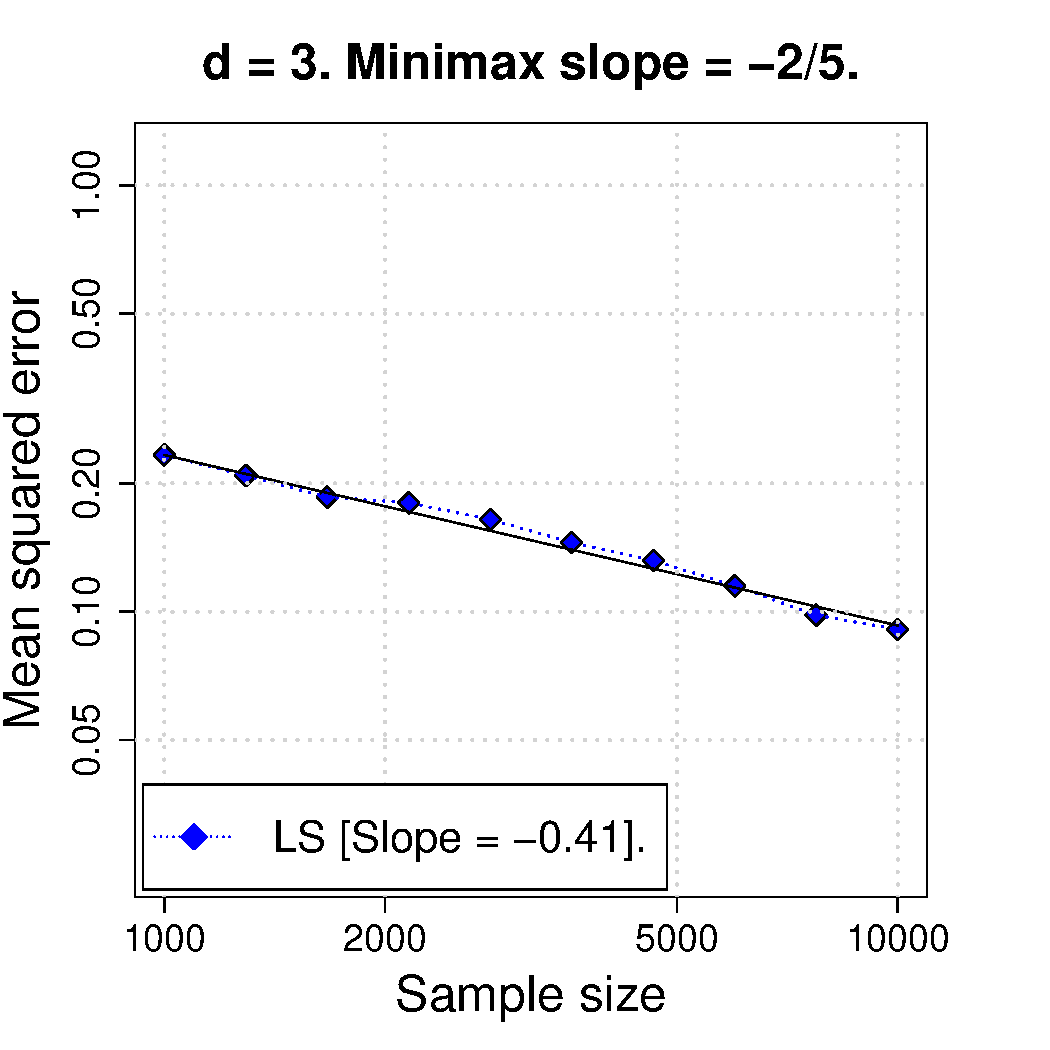
\includegraphics[width=.23\textwidth]{figures/mse_by_sample_size_3d.pdf}
	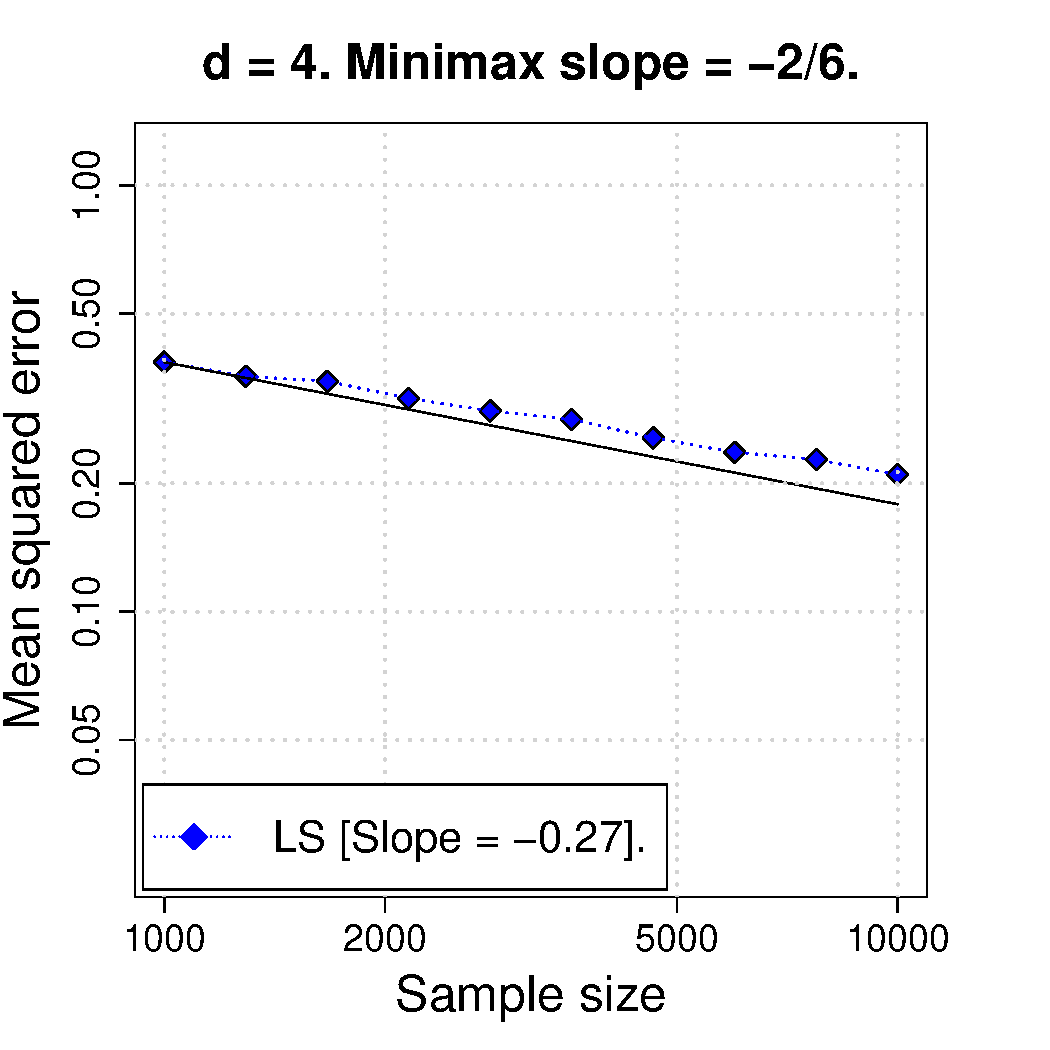
\includegraphics[width=.23\textwidth]{figures/mse_by_sample_size_4d.pdf}
	
	\caption{These are our plots.}
\end{figure}

\subsubsection{Tables}

All tables must be centered, neat, clean, and legible. Do not use hand-drawn tables.
Table number and title always appear above the table.
See Table~\ref{sample-table}.

Use one line space before the table title, one line space after the table title,
and one line space after the table. The table title must be
initial caps and each table numbered consecutively.

\begin{table}[h]
\caption{Sample Table Title} \label{sample-table}
\begin{center}
\begin{tabular}{ll}
\textbf{PART}  &\textbf{DESCRIPTION} \\
\hline \\
Dendrite         &Input terminal \\
Axon             &Output terminal \\
Soma             &Cell body (contains cell nucleus) \\
\end{tabular}
\end{center}
\end{table}

\section{SUPPLEMENTARY MATERIAL}

If you need to include additional appendices during submission, you can include them in the supplementary material file.
You can submit a single file of additional supplementary material which may be either a pdf file (such as proof details) or a zip file for other formats/more files (such as code or videos). 
Note that reviewers are under no obligation to examine your supplementary material. 
If you have only one supplementary pdf file, please upload it as is; otherwise gather everything to the single zip file.

You must use \texttt{aistats2021.sty} as a style file for your supplementary pdf file and follow the same formatting instructions as in the main paper. 
The only difference is that it must be in a \emph{single-column} format.
You can use \texttt{supplement.tex} in our starter pack as a starting point.
Alternatively, you may append the supplementary content to the main paper and split the final PDF into two separate files.

\section{SUBMISSION INSTRUCTIONS}

To submit your paper to AISTATS 2021, please follow these instructions.

\begin{enumerate}
    \item Download \texttt{aistats2021.sty}, \texttt{fancyhdr.sty}, and \texttt{sample\_paper.tex} provided in our starter pack. 
    Please, do not modify the style files as this might result in a formatting violation.
    
    \item Use \texttt{sample\_paper.tex} as a starting point.
    \item Begin your document with
    \begin{flushleft}
    \texttt{\textbackslash documentclass[twoside]\{article\}}\\
    \texttt{\textbackslash usepackage\{aistats2021\}}
    \end{flushleft}
    The \texttt{twoside} option for the class article allows the
    package \texttt{fancyhdr.sty} to include headings for even and odd
    numbered pages.
    \item When you are ready to submit the manuscript, compile the latex file to obtain the pdf file.
    \item Check that the content of your submission, \emph{excluding} references, is limited to \textbf{8 pages}. The number of pages containing references alone is not limited.
    \item Upload the PDF file along with other supplementary material files to the CMT website.
\end{enumerate}

\subsection{Camera-ready Papers}

%For the camera-ready paper, if you are using \LaTeX, please make sure
%that you follow these instructions.  
% (If you are not using \LaTeX,
%please make sure to achieve the same effect using your chosen
%typesetting package.)

If your papers are accepted, you will need to submit the camera-ready version. Please make sure that you follow these instructions:
\begin{enumerate}
    %\item Download \texttt{fancyhdr.sty} -- the
    %\texttt{aistats2021.sty} file will make use of it.
    \item Change the beginning of your document to
    \begin{flushleft}
    \texttt{\textbackslash documentclass[twoside]\{article\}}\\
    \texttt{\textbackslash usepackage[accepted]\{aistats2021\}}
    \end{flushleft}
    The option \texttt{accepted} for the package
    \texttt{aistats2021.sty} will write a copyright notice at the end of
    the first column of the first page. This option will also print
    headings for the paper.  For the \emph{even} pages, the title of
    the paper will be used as heading and for \emph{odd} pages the
    author names will be used as heading.  If the title of the paper
    is too long or the number of authors is too large, the style will
    print a warning message as heading. If this happens additional
    commands can be used to place as headings shorter versions of the
    title and the author names. This is explained in the next point.
    \item  If you get warning messages as described above, then
    immediately after $\texttt{\textbackslash
    begin\{document\}}$, write
    \begin{flushleft}
    \texttt{\textbackslash runningtitle\{Provide here an alternative
    shorter version of the title of your paper\}}\\
    \texttt{\textbackslash runningauthor\{Provide here the surnames of
    the authors of your paper, all separated by commas\}}
    \end{flushleft}
    Note that the text that appears as argument in \texttt{\textbackslash
      runningtitle} will be printed as a heading in the \emph{even}
    pages. The text that appears as argument in \texttt{\textbackslash
      runningauthor} will be printed as a heading in the \emph{odd}
    pages.  If even the author surnames do not fit, it is acceptable
    to give a subset of author names followed by ``et al.''

    %\item Use the file sample\_paper.tex as an example.

    \item The camera-ready versions of the accepted papers are 8
      pages, plus any additional pages needed for references.

    \item If you need to include additional appendices,
      you can include them in the supplementary
      material file.

    \item Please, do not change the layout given by the above
      instructions and by the style file.

\end{enumerate}

\subsubsection*{Acknowledgements}
All acknowledgments go at the end of the paper, including thanks to reviewers who gave useful comments, to colleagues who contributed to the ideas, and to funding agencies and corporate sponsors that provided financial support. 
To preserve the anonymity, please include acknowledgments \emph{only} in the camera-ready papers.


\subsubsection*{References}

References follow the acknowledgements.  Use an unnumbered third level
heading for the references section.  Please use the same font
size for references as for the body of the paper---remember that
references do not count against your page length total.

\begin{thebibliography}{}
\setlength{\itemindent}{-\leftmargin}
\makeatletter\renewcommand{\@biblabel}[1]{}\makeatother
\bibitem{} J.~Alspector, B.~Gupta, and R.~B.~Allen (1989).
    \newblock Performance of a stochastic learning microchip.
    \newblock In D. S. Touretzky (ed.),
    \textit{Advances in Neural Information Processing Systems 1}, 748--760.
    San Mateo, Calif.: Morgan Kaufmann.

\bibitem{} F.~Rosenblatt (1962).
    \newblock \textit{Principles of Neurodynamics.}
    \newblock Washington, D.C.: Spartan Books.

\bibitem{} G.~Tesauro (1989).
    \newblock Neurogammon wins computer Olympiad.
    \newblock \textit{Neural Computation} \textbf{1}(3):321--323.
\end{thebibliography}

\end{document}
